\documentclass[a4paper,11pt]{article}
\usepackage[T1]{fontenc}
\usepackage[utf8]{inputenc}
\usepackage{lmodern}
\usepackage{graphicx}
\usepackage{url}
\usepackage[colorlinks=true,urlcolor=black]{hyperref}   
\usepackage{float}     
\graphicspath{ {figures/} }



\begin{document}
\begin{center}
  \bf{Comparison of Diffrent Techques used for Email Filtering}\\
  \bf{Christopher Blackman}\\
\end{center}
\begin{abstract}
Email filtering techniques have been around for several decades. Often the major problem lies in identifying between HAM (non-junk emails), and SPAM (junk email). Often a naive Bayes classifier is enough to classify between the two distributions, however, a carful selection of words bypasses the classifier. The purpose of the experiment analyzes the use of different classifiers, and normalization techniques: Multinomial naive Bayes, Random Forest, Feed Forward Neural  Networks(FFNN), Min-Max Normalization, Principal Component Analysis(PCA) transformation. 
\end{abstract}

\section*{Theoretical}
In the experiment we use three techniques : Multinomial naive Bayes, Random Forest, and FFNN classifiers. Input data is pre-processed into word frequencies per document. We then normalize the data using three different techniques :  min-max normalization, or min-max normalization with a PCA reduction. 

Prior to feeding data into the models we preprocess data into document frequencies. The frequencies are based on the sklearn corpora of english stop words which consisted of a size of 33,485 strings. For Multinomial naive Bayes we feed only the document frequencies as 'sklearn' handled any other normalization prior to fitting. However, for the other models we used min-max normalization. Only on the FFNN did we use a combination of min-max and then PCA reduction.

The first Technique implements naive Bayes which uses Bayes' Theorem underlying concepts. Based on $x = (x_1,...,x_n)$ features it assigns probabilities for each class $p(C_k | x_1,...,x_n) = p(C_k|x)$. It then chooses the maximal probability of happening as the classification. A more common formula as seen [3]:
$$p(C_k|x) = \frac{p(C_k)p(x|C_k)}{p(x)}$$
Representing features as frequencies allows easy representation of probabilities. 

Method two used Random Forest, which represents a group of decision trees. In the training data a random subset of data is chosen in which a decision tree is constructed by choosing maximizing entropy changes. This step is repeated multiple times such that multiple trees are formed. Predictions are formed by the majority vote of all trees. Random Forest is used as a regularization technique of single decision trees due to overfitting.

Min-max normalization is a technique used as a linear transform to bound between $[-1,1]$, and represented as the following :$ \frac{X-min}{max-min}$. We used this instead of max normalization ($\frac{X}{max}$) to have a more exaggerated difference between common, and uncommon word frequencies for our weights in the FFNN. 

We also use PCA in order to project our normalized frequency vectors into a orthogonal space based on the eigenvectors. The intention was that a reduced orthogonal space would boost both time, and accuracy of the model. 
\section*{Initial Observations :}
The dataset we are working with comes from a Kaggle corpora [5], which contains a total of 5,695 emails. The dataset is split between 4,360 HAM emails, and 1,368 SPAM emails. Only subject and body are contained within the database. 

When examining corpora word frequencies, we see that there exists a separation of words between HAM and SPAM in figure [1].  Furthermore, by applying PCA reduction into a two dimensional space seen in figure [2], there exists a fairly linear separation between separation between the two sets. 

Applying k-means in a range of 1 to 60 in the 33,485 dimensional space of document frequencies fails to find a reasonable elbow point for choosing a hidden layer size as seen in figure [3]. Although there is a steep decline within the first couple of layers, and a more constant decline past layers 10 to 15.
\section*{Experiment Setup :}
We had two types FFNN with a difference of input size. Our first type had an input size of $33,485$ and used min-max normalization based off the document frequency. The Second type had a input of $1500$, and used a PCA transform on the min-max normalized document frequencies. The hidden layer used leaky rectified linear unit as the activation function, accompanied with dropout. All layers contained a bias of $0.1$, and all weights contained a standard deviation of $0.1$. We used a cross entropy loss function, and used the Adam method [6] for training gradient descent.

We trained our FFNN for 50 epocs, and using an initial learning rate of $0.5$ with a stepping function [1] on our learning rate to avoid accuracy fluxuations and overtraining. The stepping function used dropped learning rate by a half every three steps seen in figure [4].
When training we used 10-fold cross validation on the training set, but only recorded the validation set accuracy. On all models we had a validation set size of 20\% , and a training set size of 80\%. 

Multinomial Naive Bayes used the 'sklearn' implementation, with document frequency as input.
Random Forest used the 'sklearn' implementation, and used min-max normalization as input. Random Forest also had a maximum depth of a 100, and 100 estimator trees. 

\subsection*{Observations : }
The final models obtained from experimentation resulted in naive Bayes obtaining close to 99\% accuracy, and random forest/7-layer min-max FFNN obtaining close to 98\% seen in figure [6]. The larger the network size, generally lead to less accuracy. The PCA reduced networks were the worst in terms of accuracy achieving maximal of 91\%.
The general trend in the FFNN tends toward a local minimum as seen in figure [5]; however, during experimentation without a stepping function its noted that over time the models loss function would rise and, accuracy would decrease.

With regards to performance, the min-max FFNN were the worst averaging about 0.4 milliseconds per operation. Random forest obtained 0.2 milliseconds per operation. The PCA reduced FFNN obtained 0.006  milliseconds per operation, and naive Bayes about 0.001 milliseconds per operation seen in figure [7].

\subsection*{Discussion : }
The best model to choose would likely be naive Bayes. The model obtained the highest accuracy at the lowest cost per operation. Although the PCA FFNN had similar operational cost to naive Bayes, its accuracy dropped by 10\%. In contrast, the min-max FFNN and, Random Forest obtained higher accuracy at the expense of operational cost. If one wanted to improve the operational cost of Random Forest, we would recommend reducing maximal depth, or decreasing the number of decision trees. As for the FFNN, reducing operational cost is proportional to reducing dimension of search space; however, PCA FFNN shows us that reduction also losses important data characteristics. Next steps could deal with selection of a better corpora. For example removing frequencies of words where both HAM, and SPAM are common. 

\subsection*{Conclusion:}
Naive Bayes still remains the best model for email spam based on word frequencies. 
The performance and accuracy outperforms both FFNN and, Random forest.
However, email filtering does not have to be only a bag of words problem; there are plenty of metadata in emails such as : email addresses, origin, etc.  Bag of words can easily be manipulated to contain only words which are in HAM, thus passing the filter. The next possible step might be a mixture of bag of words, and blacklisting. 

\begin{figure}[H]
\centering
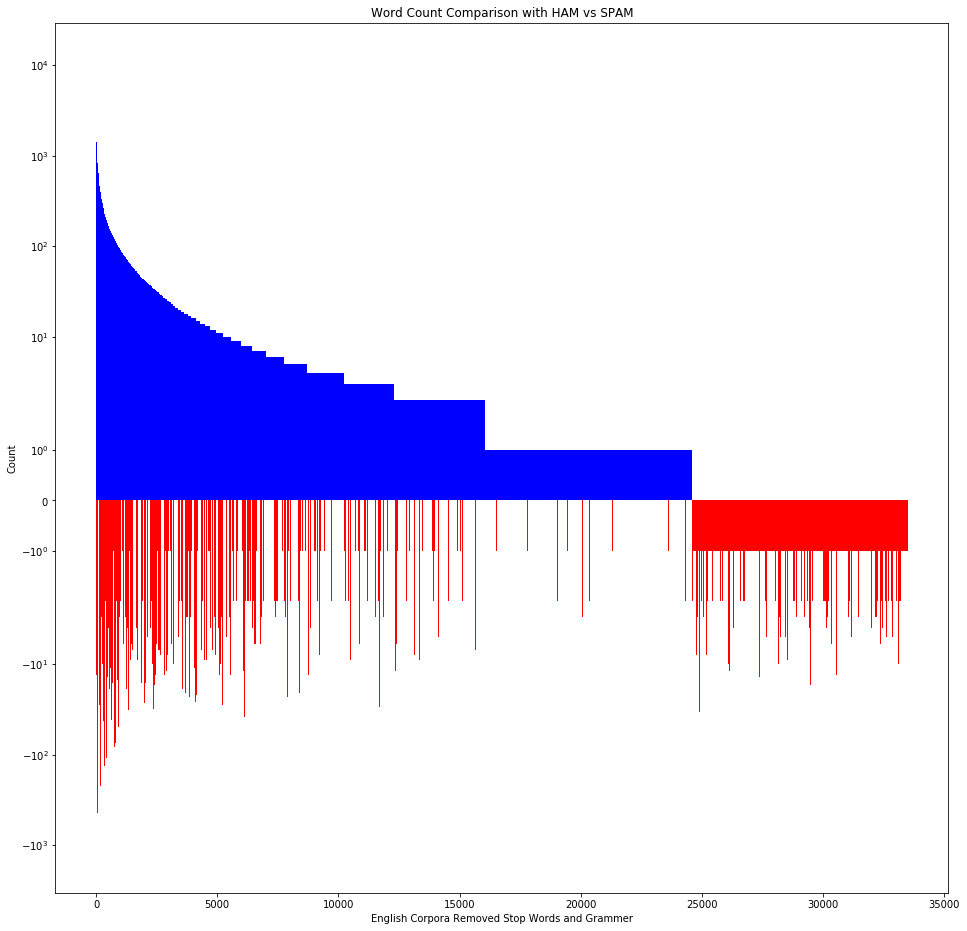
\includegraphics[width=8cm]{WordFrequency_ham_vs_spam}
\caption{}
\label{fig-1}
\end{figure}
\begin{figure}[H]
\centering
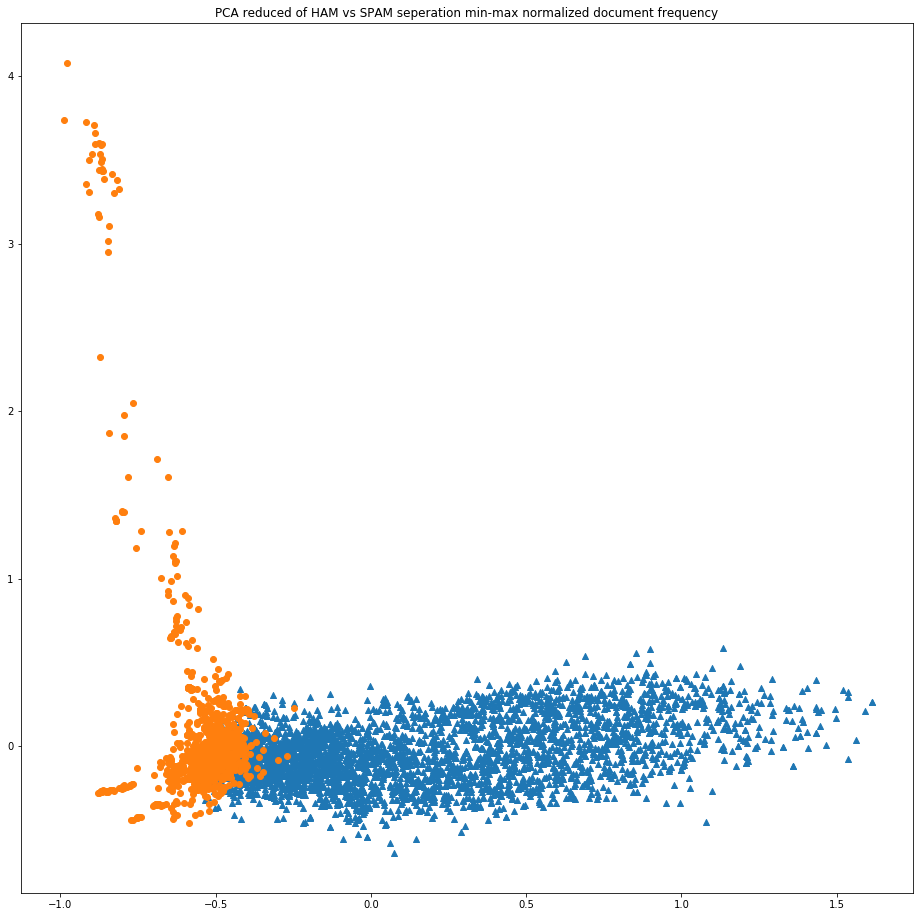
\includegraphics[width=8cm]{pca_reduction_data}
\caption{}
\label{fig-2}
\end{figure}
\begin{figure}[H]
\centering
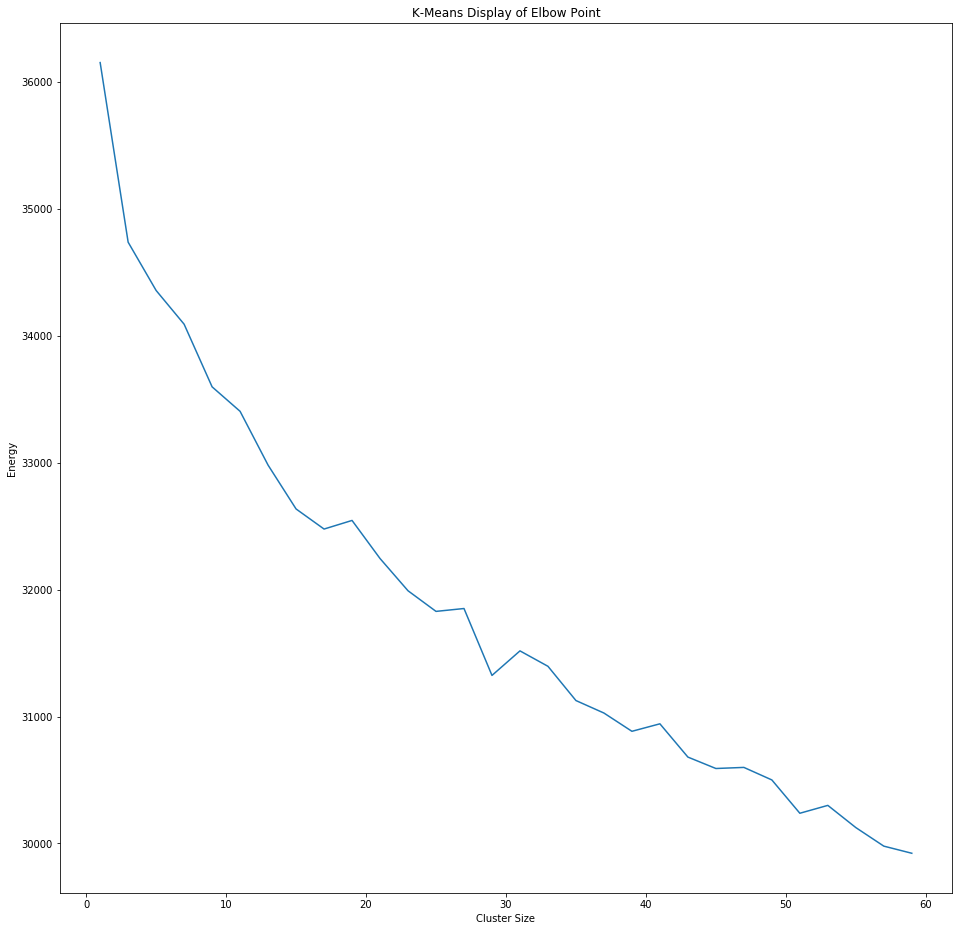
\includegraphics[width=8cm]{kmans_elbow}
\caption{}
\label{fig-3}
\end{figure}
\begin{figure}[H]
\centering
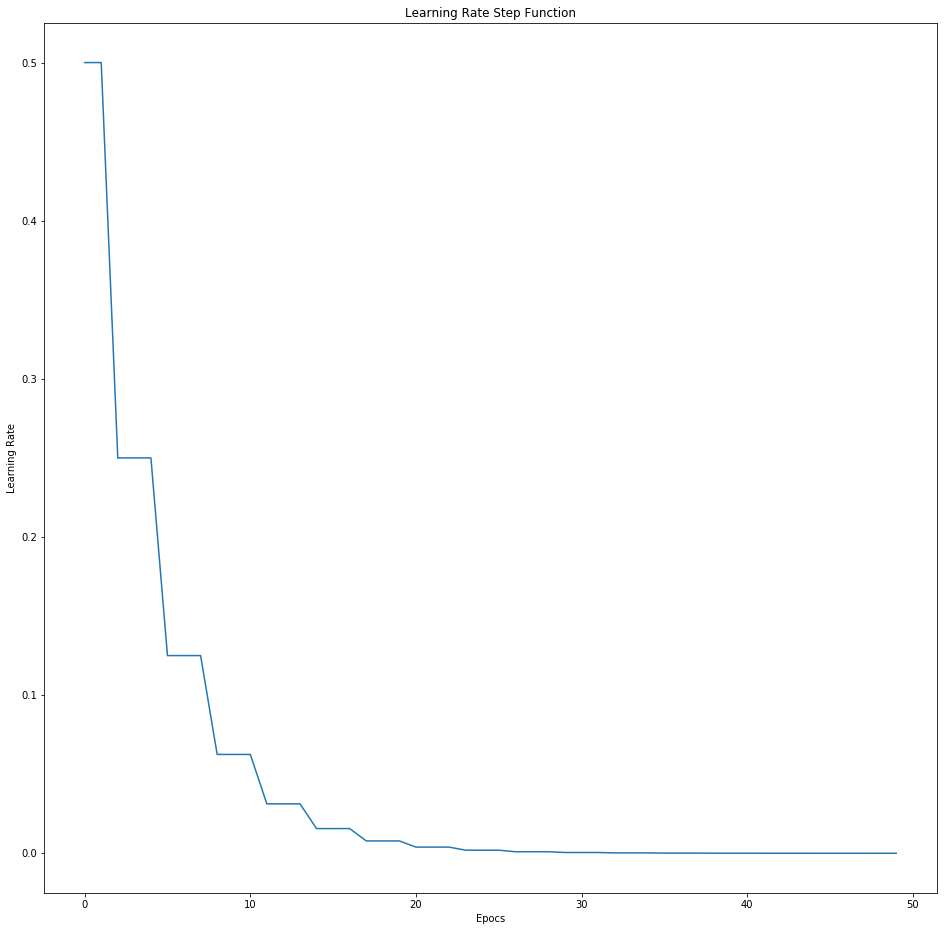
\includegraphics[width=8cm]{Step_function}
\caption{}
\label{fig-4}
\end{figure}
\begin{figure}[H]
\centering
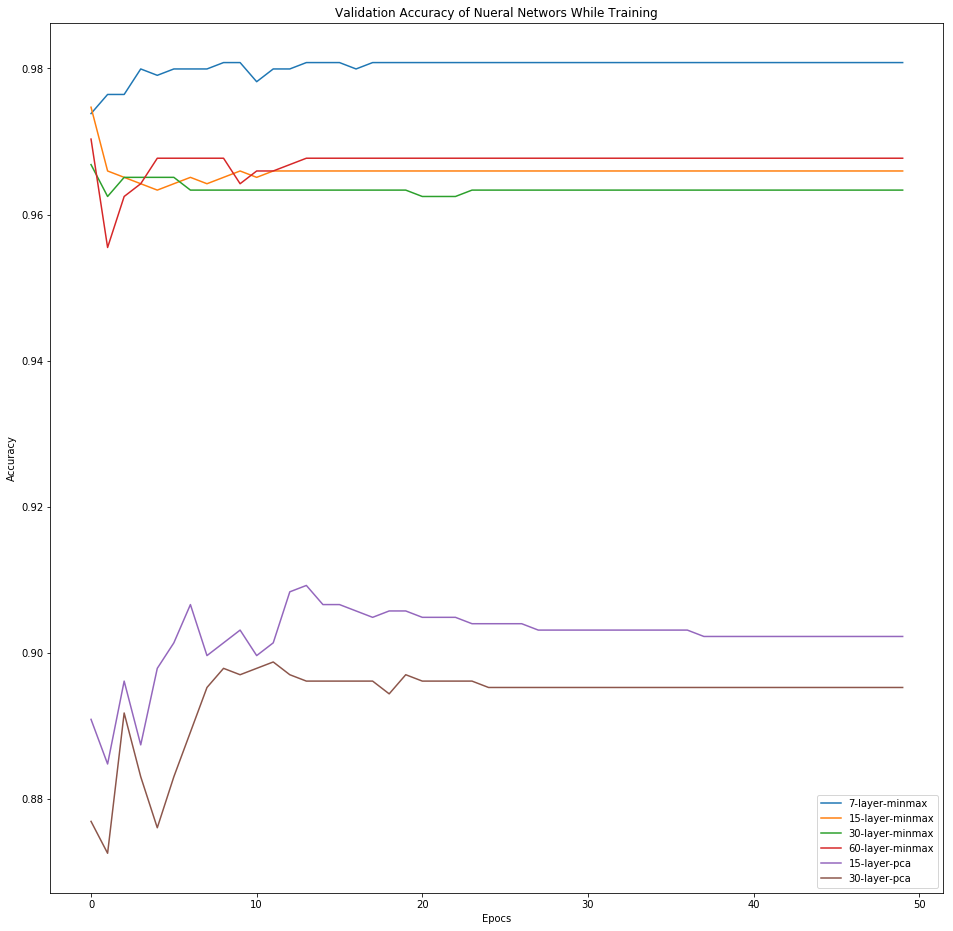
\includegraphics[width=8cm]{Training}
\caption{}
\label{fig-5}
\end{figure}
\begin{figure}[H]
\centering
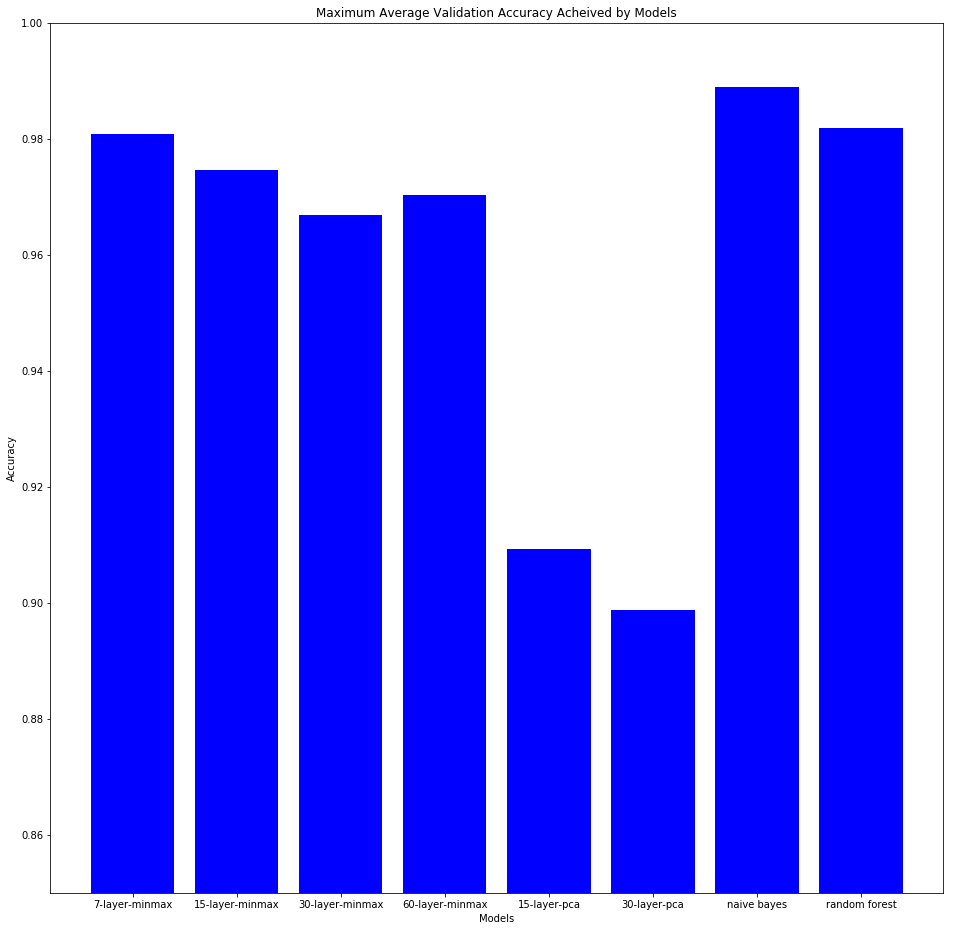
\includegraphics[width=8cm]{Accuracy}
\caption{}
\label{fig-6}
\end{figure}
\begin{figure}[H]
\centering
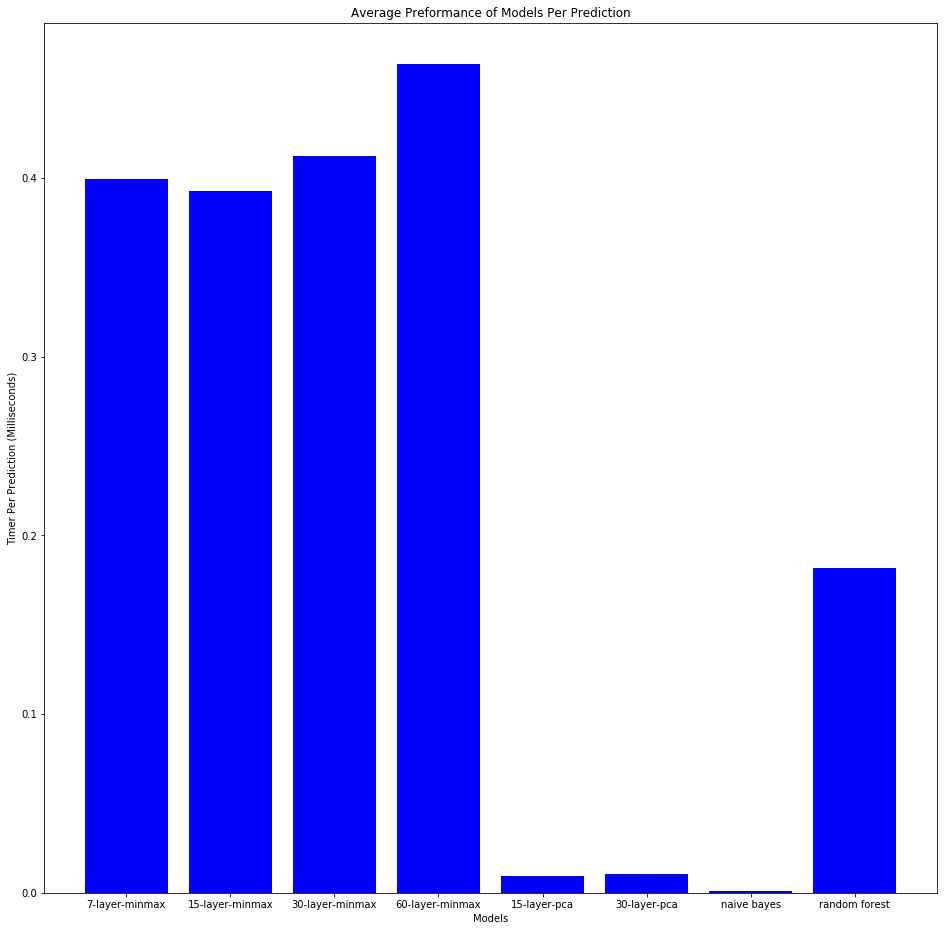
\includegraphics[width=8cm]{Preformance}
\caption{}
\label{fig-7}
\end{figure}

\begin{thebibliography}{9}
\bibitem{bib-learn_rate} 
\textit{Lau, S. (2017, July 29). Learning Rate Schedules and Adaptive Learning Rate Methods for Deep Learning. Retrieved from 
\\{\tiny\url{https://towardsdatascience.com/learning-rate-schedules-and-adaptive-learning-rate-methods-for-deep-learning-2c8f433990d1}}}
\bibitem{bib-1}
\textit{Kurenkov, A. (2016, January 13). Organizing My Emails With A Neural Net. Retrieved from \\
{\tiny\url{http://www.andreykurenkov.com/writing/ai/organizing-my-emails-with-a-neural-net/}}}
\bibitem{bib-2}
\textit{Naive Bayes classifier. (2018, November 26). Retrieved from \\
{\tiny\url{https://en.wikipedia.org/wiki/Naive_Bayes_classifier}}}
\bibitem{bib-3}
\textit{Bayesian probability. (2018, October 09). Retrieved from \\
{\tiny\url{https://en.wikipedia.org/wiki/Bayesian_probability}}}
\bibitem{bib-4}
\textit{Karthickveerakumar. (2017, July 14). Spam filter. Retrieved from\\
{\tiny\url{ https://www.kaggle.com/karthickveerakumar/spam-filter}}}
\bibitem{bib-5}
\textit{Kingma, C. P., \& Ba, J. (22 dec 2014). Adam: A Method for Stochastic Optimization. Adam: A Method for Stochastic Optimization.\\
{\tiny\url{ Retrieved from https://arxiv.org/abs/1412.6980.}}}

\end{thebibliography}


\end{document}
